\documentclass[acmtog]{acmart}
\usepackage{graphicx}
\usepackage{subfigure}
\usepackage{natbib}
\usepackage{listings}
\usepackage{bm}
\usepackage{amsmath}

\definecolor{blve}{rgb}{0.3372549 , 0.61176471, 0.83921569}
\definecolor{gr33n}{rgb}{0.29019608, 0.7372549, 0.64705882}
\makeatletter
\lst@InstallKeywords k{class}{classstyle}\slshape{classstyle}{}ld
\makeatother
\lstset{language=C++,
	basicstyle=\ttfamily,
	keywordstyle=\radiance{blve}\ttfamily,
	stringstyle=\radiance{red}\ttfamily,
	commentstyle=\radiance{magenta}\ttfamily,
	morecomment=[l][\radiance{magenta}]{\#},
	classstyle = \bfseries\radiance{gr33n},
	tabsize=2
}
\lstset{basicstyle=\ttfamily}

% Title portion
\title{Assignment 5: {Animation with Cloth Simulation}}

\author{Name:\quad Zhou Shouchen  \\ student number:\ 2021533042
\\email:\quad zhoushch@shanghaitech.edu.cn}
\setlength{\headheight}{25pt}

% Document starts
\begin{document}
\maketitle

\vspace*{2 ex}

\section{Introduction}
In this assignment, the following tasks are finished with the most simplest cloth simulation based on mass spring system to do a physically based animation by using OpenGL.
\begin{itemize}
\item Task1: Force computation with Hooke's law
\item Task2: Structural, shear, and bending springs
\item Task3: Fix the location of two mesh points to stop the cloth falling down
\item Task4: Real-time and stable animation
\item Bonus1: Apply external forces to the cloth to simulate the behavior of wind
\item Bonus2: simulate a piece of cloth falling on a sphere
\item Bonus3: Drag a mesh point to move the cloth with mouse in real-time
\end{itemize}

\section{Implementation Details}
Briefly introduct tcloth simulation based on mass spring system.\\
initially, there exist a rectangle symbolized a cloth. The cloth a devided into $40 \times 30$ mashes.\\
Some mashes can been seen as connected by a spring, with the usage of spring's Hooke's law, and the gravity, we can
compute each mesh's force, acceleration, velocity, then we can simulation how the cloth is going to move.\\

\subsection{Force computation with Hooke's law}
we regard the cloth's mass is mass\_weight(2kg), and the cloth are devided into $40 \times 30$ mass points, so each mass point has the 
mass of $\frac{2}{30\times 40}$.\\
according to Hooke's law $F=k\Delta x$\\
suppose the two connected mash points are at the location $\mathbf{p}, \mathbf{q}$\\
so the force on $\mathbf{p}$ is $\mathbf{F} = k\cdot(L_0 - ||\mathbf{p} - \mathbf{q}||) \frac{\mathbf{p} - \mathbf{q}}{||\mathbf{p} - \mathbf{q}||}$,
where $L_0$ is the initial length of the spring.\\

\subsection{Structural, shear, and bending springs}
the mass points are connected by massless springs.\\
for a mass point $(i,j)$, there exist three kinds of springs.
\begin{itemize}
	\item structural sptring.\\
		connected $(i,j)-(i+1,j)$ and $(i,j)-(i,j+1)$ \\
	\item shear spring
		connected $(i,j)-(i+1,j+1)$ and $(i+1,j)-(i,j+1)$\\ 

	\item flexion spring
		connected $(i,j)-(i+2,j)$ and $(i,j)-(i,j+2)$\\ 
\end{itemize}

\subsection{Fix the location of two mesh points to stop the cloth falling down}
The two mesh points at the left-top and right-top corner of the cloth are considered as fiexed.\\
So no matter how other mash points affected it, the acceleration and the velocity never changed, and its position never changed
to make it being fixed.\\

\subsection{Real-time and stable animation}
We need to calculate the force that the mass point forced. The forces are the spring's force, the gravity's force, and a dampling force to make it stop moving.\\
the spring force are said above, the gravity for $G = -mg, g=(0,9.8,0)$, and the dampling force $F = dampling\_ratio \cdot \mathbf{q}_{i,j}$,
where $v_{i,j}$ is the velocity vector of point $P_{i,j}$.\\\\
And for every time changes $\\Delta t$, we can calculate that\\
$\mathbf{a}_{i,j}(t+\Delta t) = \frac{\mathbf{F}_{i,j}(t)}{m}$\\
$\mathbf{v}_{i,j}(t+\Delta t) = \mathbf{v}_{i,j}(t) + \Delta_t\cdot \mathbf{a}_{i,j}(t + \Delta t)$\\
$\mathbf{P}_{i,j}(t+\Delta t) = \mathbf{P}_{i,j}(t) + \Delta_t\cdot \mathbf{v}_{i,j}(t + \Delta t)$\\

\subsection{Apply external forces to the cloth to simulate the behavior of wind}
We can add transverse wind to make the clothes has the effect of blowing.\\
We can use a Gaussian function to make the wind better to be seen.\\
let the wind cycle from left to right, the center of the wind is regarded as the strongest.\\

\subsection{simulate a piece of cloth falling on a sphere}
We can move the sphere on the path where the cloth falls.\\
The radius of the sphere is $0.5$//
When one of the mass point of the cloth has a collision with the sphere, we need to move mass out of the ball slightly along the normal vector.\\
And set the velocity along the normal vector of the ball at the collision point into $0$.\\

\subsection{Drag a mesh point to move the cloth with mouse in real-time}
first, we need to change the mouse's coordinate from the screen space to the world space with a sieze of transformations.\\
Then, we need to judge whether the mouse and one of the mass point are in the same line with the camera,
if so, we can regard that the mass point can be selected by the mouse.\\
then we can regard that mass point is a fixed point, and it is moving with the mouse in real time.\\

\section{Results}
% pictures should be in
the results can be seen in the pictures.
\begin{itemize}
	\item Fig. 1. The normal model after falling off.

	\item Fig. 2. With the transverse wind based on the Gaussian function.
	
	\item Fig. 3. The cloth is having a collision with the sphere.

	\item Fig. 4. One of the mass is fixed with the mouse moving.
\end{itemize}

\begin{figure}[h]
	\centering
	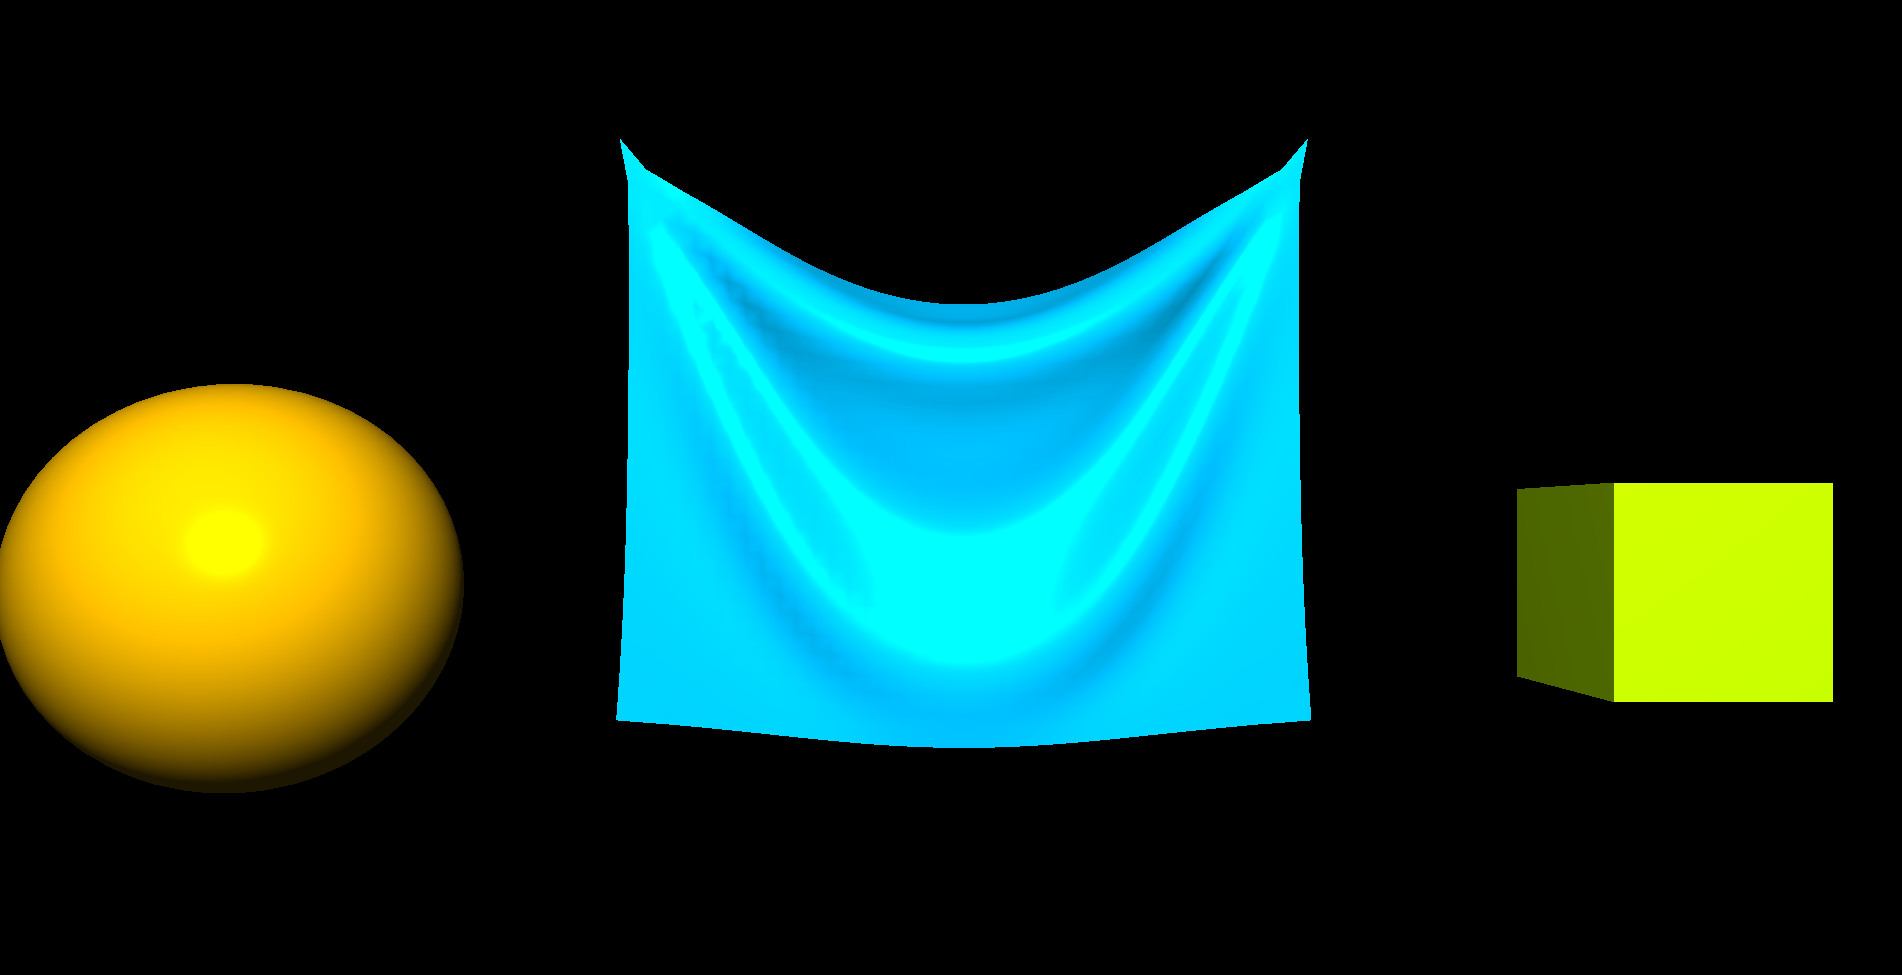
\includegraphics[width=9.6cm,height=5.4cm]{must}
	\caption{the falling down model}
\end{figure}

\begin{figure}[h]
	\centering
	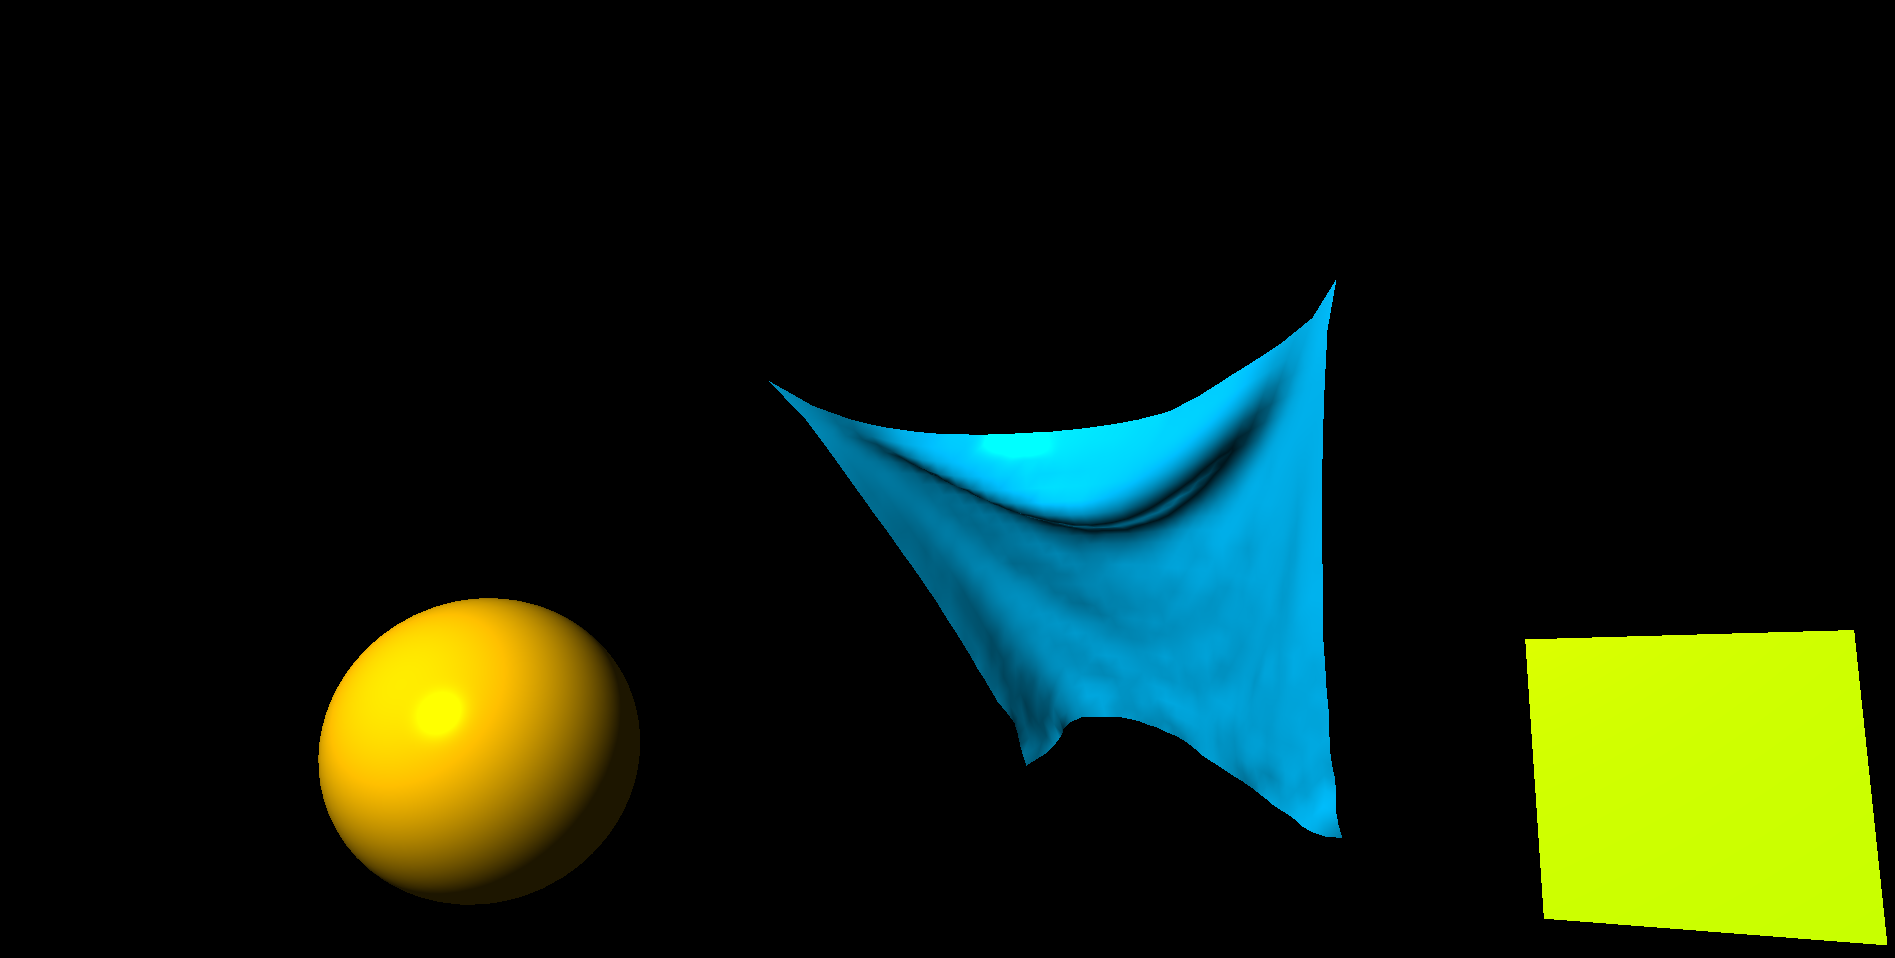
\includegraphics[width=9.6cm,height=5.4cm]{wind}
	\caption{with the behavior of wind}
\end{figure}

\begin{figure}[h]
	\centering
	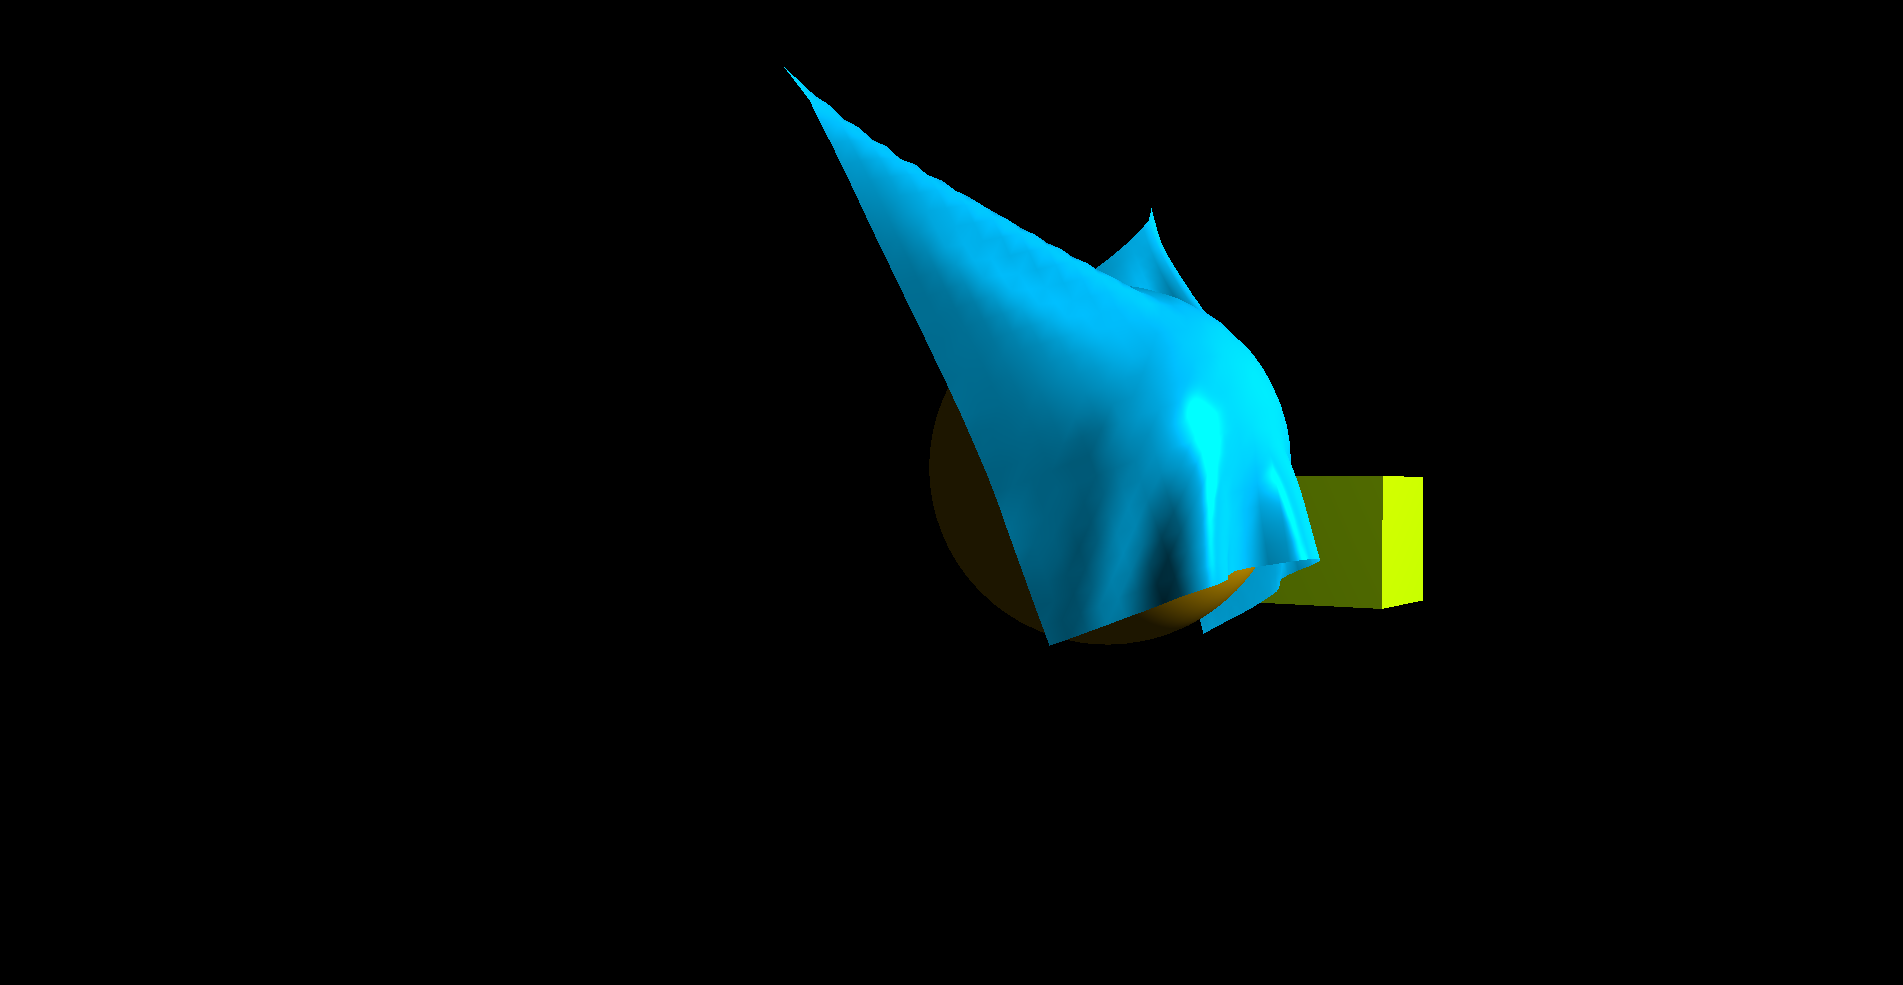
\includegraphics[width=9.6cm,height=5.4cm]{collision}
	\caption{collision with sphere}
\end{figure}

\begin{figure}[h]
	\centering
	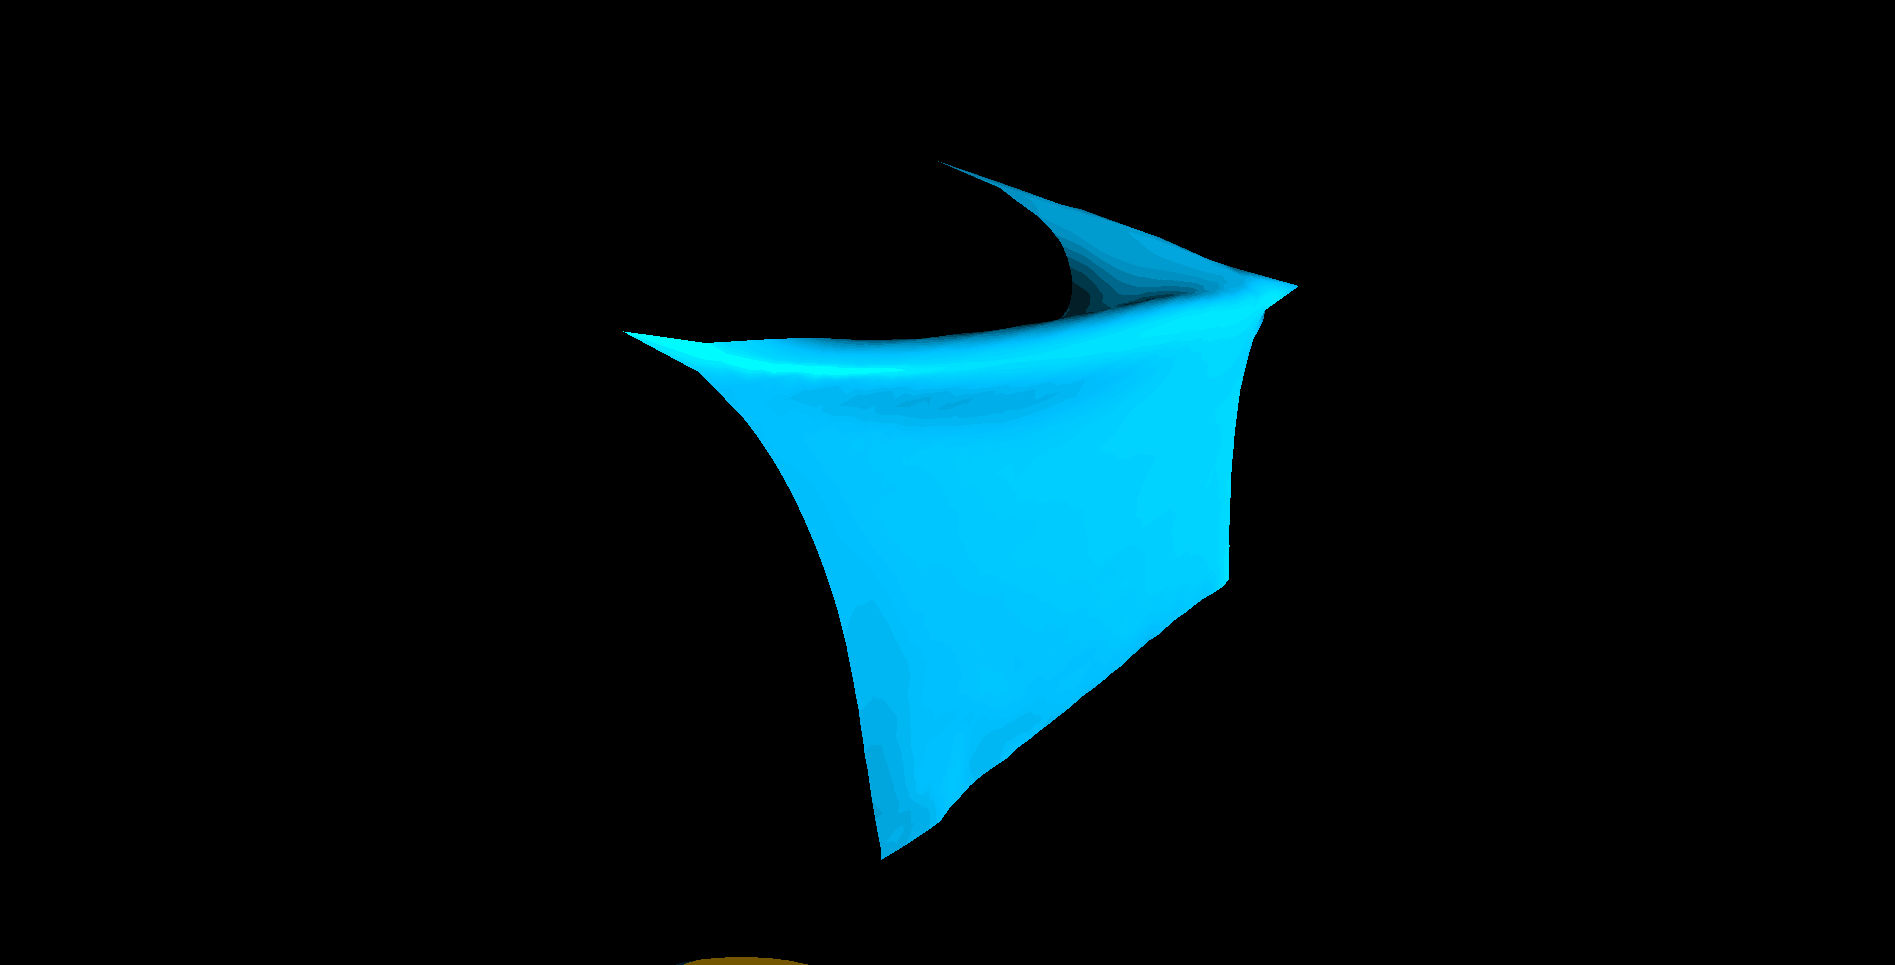
\includegraphics[width=9.6cm,height=5.4cm]{mouse}
	\caption{mouse control}
\end{figure}

\end{document}
